\documentclass[12pt,a4paper]{article}
\usepackage[utf8]{inputenc}
\usepackage[T1]{fontenc}
\usepackage{lmodern}
\usepackage[margin=1in]{geometry}
\usepackage{graphicx}
\usepackage{booktabs}
\usepackage{longtable}
\usepackage{hyperref}
\usepackage{listings}
\usepackage{xcolor}
\usepackage{enumitem}
\usepackage{tcolorbox}
\usepackage{tikz}
\usepackage{float}

\hypersetup{
    colorlinks=true,
    linkcolor=blue,
    filecolor=magenta,      
    urlcolor=cyan,
    pdftitle={Rikugan - Architecture and Design Document},
    pdfpagemode=FullScreen,
}

\lstset{
    basicstyle=\ttfamily\small,
    breaklines=true,
    frame=single,
    backgroundcolor=\color{gray!10}
}

\title{\textbf{Rikugan\\Architecture and Design Document}\\{\large Version 1.0}}
\author{}
\date{December 2025}

\begin{document}

\maketitle
\thispagestyle{empty}
\clearpage

\tableofcontents
\clearpage

\section{Introduction and Goals}

Rikugan is a gamified project management web application combining Kanban functionality with bounty-based task rewards for software development teams.

\subsection{Requirements Overview}

\textbf{Core Features:}
\begin{itemize}
    \item Role-based management: Goons (task workers), Hashira (task creators), Oyakatasama (admins)
    \item Bounty system with monetary task rewards and deadline penalties
    \item Real-time notifications and license-based access control
\end{itemize}

\subsection{Quality Goals}

\begin{table}[H]
\centering
\begin{tabular}{@{}clp{8cm}@{}}
\toprule
\textbf{Priority} & \textbf{Goal} & \textbf{Target} \\ \midrule
1 & Usability & Intuitive interface, <10min learning curve \\
2 & Security & JWT auth, RBAC, data protection \\
3 & Performance & <500ms API response, 50 concurrent users \\
4 & Maintainability & Modular architecture, 70\% test coverage \\
5 & Scalability & Support 200 users, 1000 tasks \\ \bottomrule
\end{tabular}
\caption{Quality Goals}
\end{table}

\subsection{Stakeholders}

The primary stakeholders include:
\begin{itemize}
    \item \textbf{Goons}: Junior developers who complete tasks
    \item \textbf{Hashira}: Senior developers who create and assign tasks
    \item \textbf{Oyakatasama}: System administrators with full access
\end{itemize}

\section{Architecture Constraints}

\subsection{Technical Constraints}
\begin{itemize}
    \item React 18+
    \item Node.js
    \item MySQL 8.0+
    \item Docker
    \item Web-based access
\end{itemize}

\subsection{Organizational Constraints}
\begin{itemize}
    \item 3-4 student developers
    \item One semester timeline
    \item Git version control
    \item 70\% test coverage requirement
\end{itemize}

\subsection{Conventions}
\begin{itemize}
    \item RESTful API architecture
    \item arc42 documentation standard
    \item ESLint code standards
    \item Naming conventions:
    \begin{itemize}
        \item snake\_case for database
        \item camelCase for JavaScript code
        \item PascalCase for React components
    \end{itemize}
\end{itemize}

\section{System Scope and Context}

\subsection{Business Context}

\textbf{User Roles:}

\begin{description}
    \item[Goons:] Browse and complete tasks, earn bounties
    \item[Hashira:] Create tasks, manage teams, includes all Goon functions
    \item[Oyakatasama:] Full system administration, user and license management
\end{description}

\subsection{Technical Context}

\textbf{Technical Components:}
\begin{itemize}
    \item \textbf{Frontend}: React 18+ with HeroUI (browser-based UI)
    \item \textbf{Backend}: Node.js/Express.js (RESTful API, authentication, business logic)
    \item \textbf{Database}: MySQL 8.0+ (users, tasks, bounties, notifications, licenses)
    \item \textbf{Deployment}: Docker containerization
\end{itemize}

\section{Solution Strategy}

\textbf{Architecture:} Role-based hierarchy (Goons → Hashira → Oyakatasama) + bounty incentive system

\textbf{Stack:} React 18+ (HeroUI), Node.js/Express.js (MVC), MySQL (normalized schema), Docker

\textbf{Security:} JWT authentication, RBAC at API/component levels

\textbf{Key Decisions:} Bounty-first design, license-controlled access, API-first development, audit trails

\section{Building Block View}

\subsection{System Architecture}

\begin{figure}
    \centering
    \includegraphics[width=0.75\linewidth]{high_level_block.png}
    \caption{System Architecture}
    \label{fig:placeholder}
\end{figure}

The system follows a three-tier architecture pattern(Figure 1):

\begin{itemize}
    \item \textbf{Client Layer}: React UI with HeroUI components, state management
    \item \textbf{API Gateway}: Express.js server, JWT authentication, routing, validation
    \item \textbf{Database}: MySQL with normalized schema, connection pooling
\end{itemize}

\subsection{Use Case View}

The system supports various use cases for different user roles, including task management, bounty processing, and team administration.

\subsection{Backend MVC Architecture}

\begin{description}
    \item[Model:] Data entities, business logic, database interactions
    \item[Controller:] HTTP request handling, route management
    \item[View:] JSON response formatting
\end{description}


\subsection{Backend Black Box View}

The backend system acts as a RESTful API server, exposing interfaces to the frontend and managing all business logic and data persistence.

\subsubsection*{Purpose and Responsibility}

The backend serves as the central business logic and data management layer with the following responsibilities:

\begin{itemize}
    \item \textbf{Authentication \& Authorization}: Validate user credentials, generate JWT tokens, enforce role-based access control
    \item \textbf{Data Management}: CRUD operations for all entities (users, tasks, teams, bounties, licenses)
    \item \textbf{Business Logic}: Implement bounty calculations, task lifecycle rules, deadline penalties
    \item \textbf{Notification Processing}: Generate and deliver real-time notifications for system events
    \item \textbf{License Validation}: Enforce team access control and license expiration policies
\end{itemize}

\subsubsection*{Interfaces}

\textbf{HTTP REST API Endpoints:}

\begin{table}[H]
\centering
\small
\begin{tabular}{@{}llp{6cm}@{}}
\toprule
\textbf{Endpoint} & \textbf{Methods} & \textbf{Purpose} \\ \midrule
/api/auth & POST & Login, logout, token refresh \\
/api/users & GET, POST, PUT, DELETE & User management \\
/api/tasks & GET, POST, PUT, DELETE & Task CRUD and assignment \\
/api/bounties & GET, POST & Bounty payments and history \\
/api/teams & GET, POST, PUT, DELETE & Team management \\
/api/licenses & GET, POST, PUT & License validation \\
/api/notifications & GET, PUT & Notification retrieval and updates \\ \bottomrule
\end{tabular}
\caption{Backend API Endpoints}
\end{table}

\textbf{External Dependencies:}
\begin{itemize}
    \item MySQL database connection (port 3306)
    \item Environment configuration (.env file)
    \item JWT secret keys for token signing
\end{itemize}

\subsubsection*{Quality Attributes}

\begin{itemize}
    \item \textbf{Availability}: 99\% uptime during business hours
    \item \textbf{Performance}: <500ms average response time for API calls
    \item \textbf{Scalability}: Support up to 200 concurrent users
    \item \textbf{Security}: JWT authentication, input validation, SQL injection prevention
    \item \textbf{Maintainability}: Modular architecture, 70\% test coverage
\end{itemize}

\subsection{Backend White Box View}

The backend internal structure follows the Model-View-Controller (MVC) pattern with clear separation of concerns across multiple layers.

\subsubsection*{Internal Structure}

\begin{figure}[H]
\centering
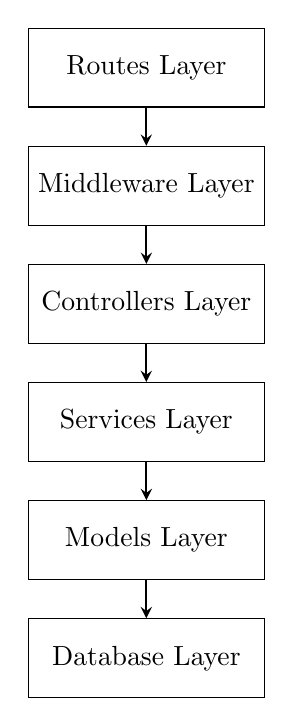
\begin{tikzpicture}[
    box/.style={rectangle, draw, minimum width=3cm, minimum height=1cm, align=center},
    arrow/.style={->, >=stealth, thick}
]
    % Layers
    \node[box] (routes) at (0,4) {Routes Layer};
    \node[box] (middleware) at (0,2.5) {Middleware Layer};
    \node[box] (controllers) at (0,1) {Controllers Layer};
    \node[box] (services) at (0,-0.5) {Services Layer};
    \node[box] (models) at (0,-2) {Models Layer};
    \node[box] (db) at (0,-3.5) {Database Layer};
    
    % Arrows
    \draw[arrow] (routes) -- (middleware);
    \draw[arrow] (middleware) -- (controllers);
    \draw[arrow] (controllers) -- (services);
    \draw[arrow] (services) -- (models);
    \draw[arrow] (models) -- (db);
\end{tikzpicture}
\caption{Backend Layered Architecture}
\end{figure}

\subsubsection*{Component Descriptions}

\begin{description}
    \item[Routes Layer] \textbf{(routes/)} \\
    Defines API endpoints and maps HTTP requests to controllers. Registers all REST routes and applies route-specific middleware.
    
    \item[Middleware Layer] \textbf{(middleware/)} \\
    Provides cross-cutting concerns:
    \begin{itemize}
        \item \texttt{auth.js}: JWT token validation and extraction
        \item \texttt{roleCheck.js}: Role-based access control enforcement
        \item \texttt{validation.js}: Request payload validation
        \item \texttt{errorHandler.js}: Global error handling and formatting
        \item \texttt{logger.js}: Request/response logging
    \end{itemize}
    
    \item[Controllers Layer] \textbf{(controllers/)} \\
    Handles HTTP requests and responses, orchestrates service calls:
    \begin{itemize}
        \item \texttt{AuthController}: Login, logout, token management
        \item \texttt{UserController}: User CRUD operations
        \item \texttt{TaskController}: Task management and assignment
        \item \texttt{BountyController}: Bounty processing and payment
        \item \texttt{TeamController}: Team operations
        \item \texttt{LicenseController}: License validation
        \item \texttt{NotificationController}: Notification delivery
    \end{itemize}
    
    \item[Services Layer] \textbf{(services/)} \\
    Implements core business logic:
    \begin{itemize}
        \item \texttt{AuthService}: Authentication, JWT generation/validation
        \item \texttt{UserService}: User management, balance updates
        \item \texttt{TaskService}: Task lifecycle, status transitions, deadline checks
        \item \texttt{BountyService}: Payment calculations, penalty processing
        \item \texttt{NotificationService}: Event-based notification generation
        \item \texttt{LicenseService}: License validation, expiration checks
    \end{itemize}
    
    \item[Models Layer] \textbf{(models/)} \\
    Data access objects (DAOs) for database operations:
    \begin{itemize}
        \item \texttt{User}: User entity CRUD
        \item \texttt{Task}: Task entity CRUD
        \item \texttt{Team}: Team entity CRUD
        \item \texttt{License}: License entity CRUD
        \item \texttt{Notification}: Notification entity CRUD
        \item \texttt{Transaction}: Transaction entity CRUD (immutable)
    \end{itemize}
    
    \item[Database Layer] \textbf{(database/)} \\
    MySQL connection management:
    \begin{itemize}
        \item \texttt{connection.js}: Connection pool configuration
        \item \texttt{migrations/}: Database schema version control
    \end{itemize}
\end{description}

\subsubsection*{Data Flow}

A typical API request flows through the system as follows:

\begin{enumerate}
    \item \textbf{Request Reception}: HTTP request arrives at Express server
    \item \textbf{Route Matching}: Router matches URL pattern to controller method
    \item \textbf{Middleware Processing}: Sequential execution of middleware chain
    \begin{itemize}
        \item Logger records request details
        \item Auth middleware validates JWT token
        \item Role check enforces permissions
        \item Validator checks request payload
    \end{itemize}
    \item \textbf{Controller Execution}: Controller receives validated request
    \item \textbf{Service Invocation}: Controller delegates to appropriate service
    \item \textbf{Business Logic}: Service executes business rules
    \item \textbf{Model Interaction}: Service calls model methods for data access
    \item \textbf{Database Operation}: Model executes SQL queries via connection pool
    \item \textbf{Response Formation}: Results propagate back through layers
    \item \textbf{JSON Response}: Controller formats and sends HTTP response
    \item \textbf{Error Handling}: Any errors caught by global error handler
\end{enumerate}

\subsubsection*{Key Design Patterns}

\begin{itemize}
    \item \textbf{Layered Architecture}: Clear separation between routes, controllers, services, and models
    \item \textbf{Dependency Injection}: Services injected into controllers, models into services
    \item \textbf{Repository Pattern}: Models act as data repositories abstracting database access
    \item \textbf{Middleware Chain}: Composable request processing pipeline
    \item \textbf{Service Layer Pattern}: Business logic isolated from HTTP concerns
    \item \textbf{Error Handling Strategy}: Centralized error handling with custom error types
\end{itemize}

\subsection{Domain Model}

\begin{figure}
    \centering
    \includegraphics[width=0.75\linewidth]{domain_model.png}
    \caption{Domain Model}
    \label{fig:placeholder}
\end{figure}

The domain model defines the core entities and their relationships within the system.

\subsection{Backend Modules}

\begin{table}[H]
\centering
\begin{tabular}{@{}lp{10cm}@{}}
\toprule
\textbf{Module} & \textbf{Responsibilities} \\ \midrule
auth & JWT authentication, login/logout, token management \\
users & User CRUD, profiles, team membership, earnings \\
tasks & Task lifecycle, assignment, status tracking \\
bounties & Payment processing, balance management, penalties \\
notifications & Event notifications, delivery, preferences \\
licenses & License validation, team access control \\
teams & Team management, member operations, statistics \\ \bottomrule
\end{tabular}
\caption{Backend Modules and Responsibilities}
\end{table}

\section{Runtime View}

\subsection{User Authentication Flow}

The authentication flow implements secure JWT-based authentication with the following steps(Figure 2):

\begin{enumerate}
    \item User submits credentials
    \item Backend validates credentials
    \item JWT token is generated and returned
    \item Token is stored on client for subsequent requests
    \item Token is validated on protected endpoints
\end{enumerate}

\begin{figure}
    \centering
    \includegraphics[width=.75\linewidth]{auth_flow.png}
    \caption{Authentication Flow}
    \label{fig:placeholder}
\end{figure}

\subsection{User Registration and Team Creation Flow}

The team creation follows these stages:

\begin{figure}
    \centering
    \includegraphics[width=0.75\linewidth]{user_registration_team_creation_flow.png}
    \caption{User Registration and Team Formation}
    \label{fig:placeholder}
\end{figure}

\subsection{Task Assignment and Completion}

The task life cycle follows these stages:

\begin{figure}
    \centering
    \includegraphics[width=0.75\linewidth]{TaskFlow.png}
    \caption{Enter Caption}
    \label{fig:placeholder}
\end{figure}

\begin{enumerate}
    \item Task creation by Hashira
    \item Task assignment to Goon
    \item Task status progression: AVAILABLE → IN\_PROGRESS → REVIEW → COMPLETED
    \item Bounty distribution upon completion
\end{enumerate}

\subsection{Notification System Flow}

Real-time notifications(Figure 4) keep users informed of:
\begin{itemize}
    \item Task assignments
    \item Status changes
    \item Bounty payments
    \item Deadline reminders
\end{itemize}

\begin{figure}
    \centering
    \includegraphics[width=0.75\linewidth]{notification_flow.png}
    \caption{Notification Flow}
    \label{fig:placeholder}
\end{figure}

\subsection{License Validation and Team Access Control}

License validation(Figure 5) ensures:
\begin{itemize}
    \item Valid team licenses
    \item User count within limits
    \item Active license status
    \item Expiration monitoring
\end{itemize}

\begin{figure}
    \centering
    \includegraphics[width=0.75\linewidth]{license_flow.png}
    \caption{License Flow}
    \label{fig:placeholder}
\end{figure}

\section{Deployment View}

\begin{figure}
    \centering
    \includegraphics[width=0.75\linewidth]{deployment.png}
    \caption{Deployment Diagram with Docker}
    \label{fig:placeholder}
\end{figure}

\textbf{Components:}
\begin{itemize}
    \item \textbf{Frontend Container}: React 18+/Vite (production build)
    \item \textbf{Backend Container}: Node.js 18+/Express.js (API server)
    \item \textbf{Database Container}: MySQL 8.0+ (persistent storage)
    \item \textbf{Reverse Proxy}: nginx (load balancing, SSL)
\end{itemize}

\textbf{Requirements:}
\begin{itemize}
    \item Docker 20.10+
    \item Docker Compose 2.0+
    \item 4GB RAM
    \item 20GB disk space
\end{itemize}


\section{Quality Scenarios}

\subsection{Quality Tree}

\begin{tcolorbox}[title=Rikugan Quality Goals]
\textbf{Usability}
\begin{itemize}[leftmargin=2em]
    \item \textit{Learning Curve (High Priority)}\\
    New users can complete basic tasks within 10 minutes
    \item \textit{Interface Consistency (Medium Priority)}\\
    All pages follow consistent navigation patterns
\end{itemize}

\textbf{Performance}
\begin{itemize}[leftmargin=2em]
    \item \textit{Response Time (High Priority)}\\
    API calls respond within 500ms for 95\% of requests
    \item \textit{Concurrent Users (Medium Priority)}\\
    Support 50 simultaneous users without degradation
\end{itemize}

\textbf{Security}
\begin{itemize}[leftmargin=2em]
    \item \textit{Authentication (High Priority)}\\
    Secure login with role-based access control
    \item \textit{Data Protection (High Priority)}\\
    All user data encrypted and validated
\end{itemize}

\textbf{Maintainability}
\begin{itemize}[leftmargin=2em]
    \item \textit{Code Quality (Medium Priority)}\\
    70\% test coverage with clean architecture
    \item \textit{Documentation (Medium Priority)}\\
    Complete API and component documentation
\end{itemize}
\end{tcolorbox}

\vspace{2em}
\hrule
\vspace{1em}
\noindent\textbf{Document:} Architecture design per arc42 template \\
\textbf{Version:} 1.0 \\
\textbf{Updated:} December 2025

\end{document}
